\documentclass[10pt,xcolor=dvipsnames]{beamer}

\usetheme{metropolis}%default}%simple}

\usepackage{lmodern}
%\usepackage[scale=2]{ccicons}
\usepackage{ccicons}


\usepackage{graphicx}
\usepackage{amsmath,amssymb}
%\usepackage{colortbl}
%\usepackage{color}
\usepackage{algorithm}
\usepackage{algorithmic}
\usepackage{amsthm}
\usepackage{mathtools}   %:= symbol
\usepackage{multirow}
\usepackage{rotating}
%\usepackage[round]{natbib}
%\usepackage[version=0.96]{pgf}
\usepackage{tikz}
\usepackage{tikz-3dplot}
\usetikzlibrary{matrix,calc,shapes,shadows,arrows,positioning,fit}
\definecolor{cof}{RGB}{219,144,71}
\definecolor{greeo}{RGB}{91,173,69}
\tdplotsetmaincoords{70}{165}

\usepackage{amsmath,amsfonts,amscd,amssymb}
%\usepackage[francais]{babel}
%\usepackage[francais]{layout}
\usepackage[english]{babel}
\usepackage[english]{layout}
%\usepackage[utf8]{inputenc}
%\usepackage{nantes_theme}
%\usepackage{multirow}
\usetikzlibrary{calc,3d}
\usepackage{appendixnumberbeamer}

\DeclareMathOperator{\conv}{\rm conv}
\DeclareMathOperator{\cl}{\rm cl}
\newcommand{\mR}{\mathbb{R}}
\newcommand{\mN}{\mathbb{N}}
\newcommand{\mZ}{\mathbb{Z}}
\newcommand{\mB}{\{0,1\}}
\newcommand{\red}{\textcolor{red}}
\newcommand{\blue}{\textcolor{blue}}
\newcommand{\magenta}{\textcolor{magenta}}

\newcommand{\orange}{\textcolor{orange}}


%
\newcommand{\R}{\mathbb{R}}%Mengen R
\newcommand{\N}{\mathbb{N}}
\newcommand{\Z}{\mathbb{Z}}
\newcommand{\Q}{\mathbb{Q}}
\newcommand{\B}{\mathbb{B}}
\newcommand{\ab}{\par\noindent}%Absatz ohne Einzug
%


%
%\usepackage{microtype}%Zeilenumbruchverbesserung
%\usepackage[T1]{fontenc}%Kodierung der Ausgabe

%\usepackage{biblatex}%Literaturverzeichnis, falls notwendig. Ansonsten auskommentieren
%\addbibresource{Literatur.bib}%Name des Literaturverzeichnises hier einfügen!!!

\usepackage{url}%Anklickbare URL im pdf
%\usepackage{hyperref}%Anklickbare Kapitel im Inhaltsverzeichnis und anklickbare Referenzen; beides im pdf

%\graphicspath{{pictures/}}%Pfad, in dem die Bilder gespeichert sind: Im Unterordner bilder

\usepackage{tabularx}%Tabellen
\usepackage{booktabs}%Verbesserungen und andere Kommandos für Tabellen

\usepackage{units} %Weiteres Mathepaket mit \nicefrac{Zähler}{Nenner} Umgebung für Brüche
\usepackage{eurosym}%Eurozeichen
%\usepackage{csquotes} %Anführungszeichen

%\usepackage{algpseudocode} %Algorithmen

%\usepackage{pgfplots}%Plots
%\usepgfplotslibrary{dateplot}

\usepackage{xcolor}%mehr Farben
\usepackage{BeamerColor}

\usepackage{xspace}

\usepackage{todonotes}
\usepackage{caption}
\usepackage{subcaption}


\usetikzlibrary{mindmap}


%
% --- Tikz definitions from Stefan
%
\colorlet{boxfill}{black!10}
\colorlet{boxhead}{black!20}
\colorlet{boxdraw}{black!70}
\colorlet{linescolor}{black!70}
\tikzstyle{boxstyle}=[draw=boxdraw,text=black,thick,rounded corners]
\tikzstyle{taskbox}=[boxstyle,rectangle,text width=3cm,rectangle split,rectangle split parts=2,
                     rectangle split part fill={boxhead,boxfill}]
\tikzstyle{line}=[very thick,linescolor,rounded corners]

%
% --- 1st slide
%

\title{{{\large vOptSolver, \vspace{-0mm}\\ 
a ``get and run'' solver of multiobjective linear \vspace{-2mm}\\
 optimization problems  built on Julia and JuMP}}}
\subtitle{\scriptsize{MCDM'2017: 24th International Conference on Multiple Criteria Decision Making \vspace{-2mm}\\%
July 10 -- 14, 2017. Ottawa, Canada}}
\date{\today}
\author{Xavier GANDIBLEUX$^1$, 
Gauthier SOLEILHAC$^1$, 
Flavien    LUCAS$^1$,\\
Anthony    PRZYBYLSKI$^1$,
Stefan    RUZIKA$^2$,
Pascal    HALFFMANN$^2$}
\institute{Universit\'e de Nantes, France$^1$ -- University of Koblenz-Landau, Germany$^2$}



\begin{document}


\maketitle

% ================================================================
\begin{frame}{}

\vspace{6mm}
{\Large \textbf{vOpt} Research Project}

\footnotesize{
Exact Efficient Solution of Mixed Integer Programming Problems with Multiple Objective Functions}
%
(ANR/DFG-14-CE35-0034-01)


\vspace{8mm}
%\begin{center}
  
\includegraphics{logovopt5.jpg}
\vspace{8mm}


%\bigskip

\footnotesize{
Parts (algorithms, instances) of the outputs are integrated in:
\begin{itemize}
\item \textbf{vOptSolver}: a solver of multiobjective linear optimization problems (MOCO, MOIP, \orange{MOMILP}, MOLP)
\vspace{3mm}

\item \textbf{vOptLib}: a numerical instances library of multiobjective linear optimization problems (MOCO, MOIP, \orange{MOMILP}, MOLP)\\
\smallskip
History: MCDMlib (opened in 1998) --- MOCOlib, the MOCO section of the MCDMlib (opened in 2007) --- GUEPARDlib (opened in 2010)


\end{itemize}
}

\end{frame}

% ================================================================

\begin{frame}{Content}

\tableofcontents

\end{frame}

% ================================================================
% ================================================================
% ================================================================
\section{1. Introduction}

% ================================================================
\begin{frame}{Context}

\hspace{-3mm}Computing $Y_N$ for Multiobjective linear Optimization Problems (MOP):


\begin{columns}
\begin{column}{0.33\textwidth}
$$
\begin{array}{rcl}
\min z(x) & = & {C}x\\
\hbox{s/t } Tx & \leqq & d\\
x & \in & 
\mR^{n_1} \times \mZ^{n_2}
\notag
\end{array}
\vspace{2mm}
$$
\begin{center}
Multi Objective Mixed-Integer Linear Problem (MOMILP)
\end{center}
\end{column}
\begin{column}{0.33\textwidth}
$$
\begin{array}{rcl}
\min z(x) & = & {C}x\\
\hbox{s/t } Tx & \leqq & d\\
x & \in & 
\mR^{n_1}
\notag
\end{array}
\vspace{2mm}
$$
\begin{center}
Multi Objective\\ Linear \\Problem (MOLP)
\end{center}
\end{column}
\begin{column}{0.33\textwidth}
$$
\begin{array}{rcl}
\min z(x) & = & {C}x\\
\hbox{s/t } Tx & \leqq & d\\
x & \in & 
\mZ^{n_2}
\notag
\end{array}
\vspace{2mm}
$$
\begin{center}
Multi Objective\\ Integer \\Problem (MOIP)
\end{center}
\end{column}
\end{columns}
\vspace{2mm}

\begin{center}
MO(M)ILP + structure\\
MultiObjective Combinatorial Optimization (MOCO)
\end{center}
\vspace{2mm}
\noindent 
where:
\vspace{-6mm}
%\vfill
$$
\begin{array}{rcl}
%\only<1-2>{\blue{x \in \mR^{n_1} \times \mZ^{n_2}}
%& \longrightarrow & n=n_1+n_2 \hbox{ variables, } j = 1,\ldots,n\\}
%\only<3>{\blue{x \in \mR^{n_1}}
%& \longrightarrow & n=n_1+n_2 \hbox{ variables, } j = 1,\ldots,n\\}
%\only<4>{\blue{x \in \mZ^{n_2}}
%& \longrightarrow & n=n_1+n_2 \hbox{ variables, } j = 1,\ldots,n\\}
T \in \mZ^{m \times n} & \longrightarrow & m \hbox{ constraints, } i = 1,\ldots,m\\
%
C \in \mZ^{n\times p} & \longrightarrow & \hbox{the objective matrix}\\
%\only<2>{\red {C \in \mZ^{n\times p}} & \red {\longrightarrow} & \hbox{\red {the objective matrix}}\\}
%\only<3->{C \in \mZ^{n\times p} & \longrightarrow & \hbox{the objective matrix}\\}
%
X=\{x \in \mR^{n_1} \times \mZ^{n_2}| Tx\leq d\}\subseteq\mR^n  & \longrightarrow & \hbox{the set of feasible solutions}\\
Y=z(X)\subseteq \mR^p & \longrightarrow & \hbox{the set of images}\\
\notag
\end{array}
$$


\end{frame}


% ================================================================
\begin{frame}{Identified software for computing exact $Y_N$ of MOP}


\begin{itemize}
  \item \textbf{ADBASE} (Ralph Steuer, 1975)
    \begin{itemize}
      \item       {\footnotesize Problem class solved: MOLP}
      \item       {\footnotesize Algorithm(s): simplex algorithm}
      \item       {\footnotesize not available online}
    \end{itemize}
    \vspace{3mm}
%    
  \item \textbf{Bensolve} (Andreas L\"ohne, 2017); available online:
 
    \begin{itemize}
      \item       {\footnotesize Problem class solved: vector linear programs (including MOLP)}
      \item       {\footnotesize Algorithm(s): Benson's algorithm (language C)}
      \item       {\footnotesize \url{http://bensolve.org}}
    \end{itemize}
     \vspace{3mm}    
%
  \item \textbf{Inner} (Laszlo Csirmaz, 2016); available online:
    \begin{itemize}
      \item       {\footnotesize Problem class solved: MOLP}
      \item       {\footnotesize \url{https://github.com/lcsirmaz/inner}}
    \end{itemize}
     \vspace{3mm}    
%
  \item \textbf{PolySCIP} (Sebastian Schenker, 2016); available online:
    \begin{itemize}
      \item       {\footnotesize Problem classes solved: $p$-LP, $2$-IP, $3$-IP (MOMILP experimentally)}
      \item       {\footnotesize  \url{http://polyscip.zib.de} }
    \end{itemize}
\end{itemize}

\end{frame}

% ================================================================
\begin{frame}{Presentation of vOptSolver (1/2)}

\begin{itemize}
\item Aims

\begin{itemize}
    \item Solver of multiobjective linear optimization problems for scientifics and practionners
    \item Easy to formulate a problem, to provide data, to solve a problem, to collect the outputs, to analyze the solutions
    \item Natural and intuitive use for mathematicians, informaticians, engineers
\end{itemize}
\medskip

\item Purposes

\begin{itemize}
    \item Solving needs:\\ methods and algorithms for performing numerical experiments
    \item Research needs:\\ support and primitives for the development of new algorithms
    \item Pedagogic needs:\\ environment for practicing of theories and algorithms
\end{itemize}

%\item Characteristics
%
%\begin{itemize}
%    \item Efficient, flexible, evolutive solver
%    \item Free, open source, multi-platform, reusing existing specifications
%    \item Easy installation, no need of being expert in computer science
%\end{itemize}
%
%\item Background
%
%\begin{itemize}
%    \item Julia programming language
%    \item JuMP algebraic language
%    \item Usual free (GLPK) and commercial (CPLEX, GUROBI) MILP solvers
%\end{itemize}

\end{itemize}

\end{frame}

% ================================================================
\begin{frame}{Presentation of vOptSolver (2/2)}

\begin{itemize}
%\item Aims
%
%\begin{itemize}
%    \item Solver of multiobjective linear optimization problems for scientifics and practionners
%    \item Easy to formulate a problem, to provide data, to solve a problem, to collect the outputs, to analyze the solutions
%    \item Natural and intuitive use for mathematicians, informaticians, engineers
%\end{itemize}
%
%\item Purposes
%
%\begin{itemize}
%    \item Solving needs: methods and algorithms for performing numerical experiments
%    \item Research needs: support and primitives for the development of new algorithms
%    \item Pedagogic needs: environment for practicing of theories and algorithms
%\end{itemize}

\item Characteristics

\begin{itemize}
    \item Efficient, flexible, evolutive solver
    \item Free, open source, multi-platform, reusing existing specifications
    \item Easy installation, no need of being expert in computer science
\end{itemize}
\medskip

\item Background

\begin{itemize}
    \item Julia programming language, and JuMP algebraic language
    \item Usual free (GLPK) and commercial (CPLEX, GUROBI) MILP solvers
    \item homemade solvers implemented in C/C++ language 
\end{itemize}

\end{itemize}

\begin{center}
\textbf{
 vOptSolver\\ $\sim$\\ a backbone, \\  based on Julia and JuMP, \\ embedding algorithms coded in C/C++/Julia
 }
\end{center}
\end{frame}

% ================================================================
\begin{frame}{Why Julia and JuMP as cement of vOptSolver?}

%\begin{itemize}
%\item 
\textbf{Julia programming language}
\begin{itemize}
\footnotesize{
    \item a high-level, high-performance programming language for scientific computing\vspace{-1mm}
    \item familiar for the practitioners of Matlab, Fortran, Python, C/C++, Pascal, etc.\vspace{-1mm}
    \item integrates natively a wrapper to external programs written in C or C++ \vspace{-1mm}
    \item  \url{http://julialang.org/}
}
\end{itemize}

\medskip

%\item 
\textbf{JuMP algebraic language} (Julia for mathematical optimization)
\begin{itemize}
\footnotesize{
    \item a domain-specific modeling language for mathematical optimization in Julia\vspace{-1mm}
    \item familiar for the practitioners of GMP, AMPL, MPL, GAMS, OPL, and etc.\vspace{-1mm}
    \item wrapped with several open-source/commercial solvers (e.g. GLPK and CPLEX).\vspace{-1mm}
    \item  \url{http://jump.readthedocs.io/en/latest/}
    }
\end{itemize}

%\end{itemize}
\medskip

More:\\
\footnotesize{
Miles Lubin and Iain Dunning:
Computing in Operations Research Using Julia.
\textit{INFORMS Journal on Computing} 27:2 , 238-248, 2015.}
    
\end{frame}



% ================================================================
% ================================================================
% ================================================================
\section{2. vOptSolver}

%
% ================================================================
% 
\begin{frame}{Multi-objective linear optimization problems targeted}

{\footnotesize
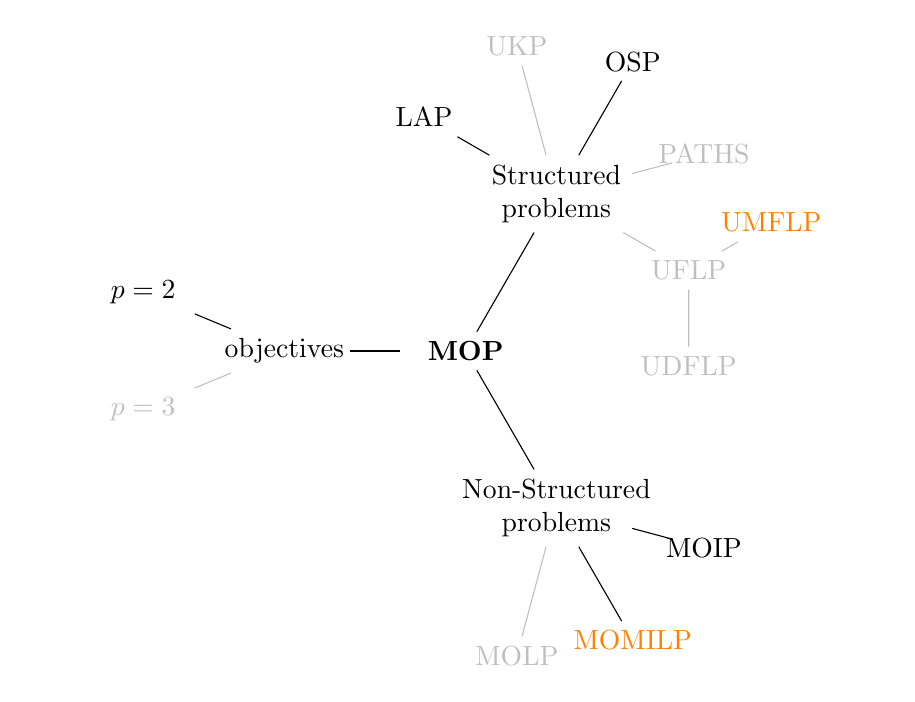
\begin{tikzpicture}[scale=0.485, grow cyclic, text width=2.7cm, align=flush center,
    level 1/.style={level distance=4.75cm,sibling angle=120},
    level 2/.style={level distance=4.0cm,sibling angle=45},
    level 3/.style={level distance=2.5cm,sibling angle=120}]
\node{\normalsize{\textbf{MOP}}}
   child [color=white]{ }
   child { node {Non-Structured\\ problems}
        child [color = black!25]{ node {MOLP}}
        child { node {\orange{MOMILP}}}
        child { node {MOIP}}
    }
    child { node {Structured\\ problems}
        child [color = black!25]{ node {UFLP} 
          child { node {UDFLP}}
          child { node {\orange{UMFLP}}}
          }
        child [color = black!25]{ node {PATHS}}
        child [color = black]{ node {OSP}}
        child [color = black!25]{ node {UKP}}        
        child { node {LAP}}
    }
    child { node {objectives}
        child { node {$p=2$}}
        child [color = black!25]{ node {$p=3$}}
%        child [concept color=green!40]{ node {Themes and Handouts}}
    };


\end{tikzpicture}
\bigskip

\vspace{-15mm}{\orange{Framework of the\\ ANR/DFG research project}}
}

\end{frame}



% ================================================================
\begin{frame}{Design of {vOptSolver}}

\hspace{-18mm}
%\begin{center}
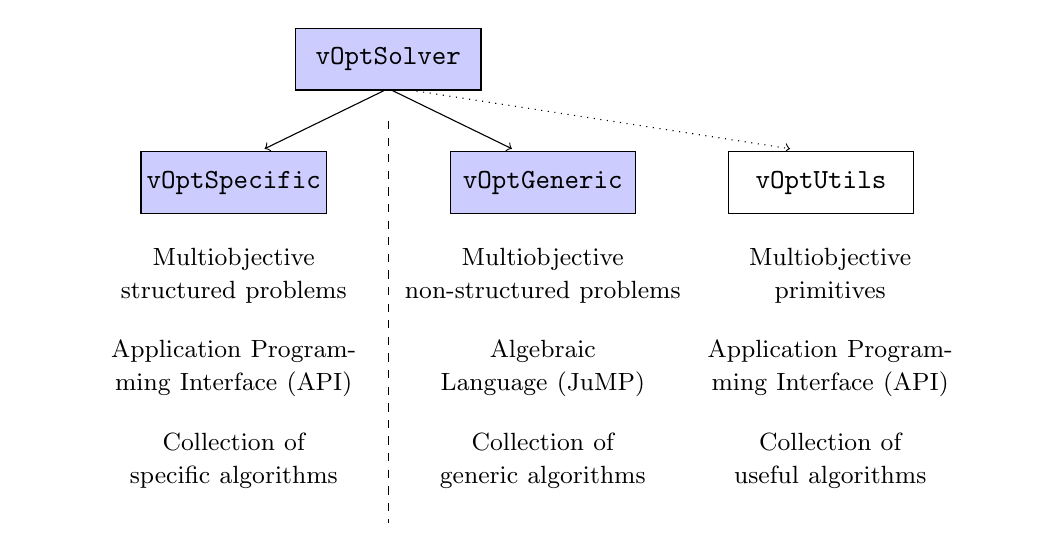
\begin{tikzpicture}[scale=0.785]%[auto]

\draw [fill=blue!20] (4,12) rectangle (7,13);
\node [text width=8cm,text centered] at (5.5,12.5) {\texttt{vOptSolver}};

\draw [->] (5.45,12) -- (3.5,11.05);
\draw [->] (5.55,12) -- (7.5,11.05);
\draw [->, dotted] (5.85,12) -- (12,11.05);

\draw [fill=blue!20] (1.5,10) rectangle (4.5,11);
\node [text width=5cm,text centered] at (3,10.5) {\texttt{vOptSpecific}};
\draw [fill=blue!20] (6.5,10) rectangle (9.5,11);
\node [text width=5cm,text centered] at (8,10.5) {\texttt{vOptGeneric}};
\draw [fill=white!20] (11,10) rectangle (14,11);
\node [text width=5cm,text centered] at (12.5,10.5) {\texttt{vOptUtils}};

\draw  [dashed](5.5,11.5) -- (5.5,5);

\node [text width=4cm,text centered] at (3,9) {\small Multiobjective \\ structured problems};
\node [text width=4cm,text centered] at (3,7.5) {\small Application Programming Interface (API)};
\node [text width=4cm,text centered] at (3,6) {\small {Collection of \\ specific algorithms}};
%\node [text width=4cm,text centered, color=Gray] at (3,4.5) {\footnotesize \texttt{Pkg.Add(vOptSpecific.jl)}};

\node [text width=4cm,text centered] at (8,9) {\small Multiobjective \\ non-structured problems};
\node [text width=4cm,text centered] at (8,7.5) {\small Algebraic\\ Language (JuMP)};
\node [text width=4cm,text centered] at (8,6) {\small {Collection of \\ generic algorithms}};
%\node [text width=4cm,text centered, color=Gray] at (8,4.5) {\footnotesize \texttt{Pkg.Add(vOptGeneric.jl)}};

\node [text width=4cm,text centered] at (12.65,9) {\small Multiobjective \\ primitives};
\node [text width=4cm,text centered] at (12.65,7.5) {\small Application Programming Interface (API)};
\node [text width=4cm,text centered] at (12.65,6) {\small {Collection of \\ useful algorithms}};
%\node [text width=4cm,text centered, color=Gray] at (12.65,4.5) {\footnotesize \texttt{Pkg.Add(vOptUtils.jl)}};

\end{tikzpicture}
%\end{center}

\end{frame}


%
% ================================================================
% 
\begin{frame}{Using vOptSolver}

vOptSolver has been tested with:
\begin{itemize}
\item Julia v0.6
\item GLPK v4.62
\end{itemize}
\bigskip

Two modes:\\ 
\begin{enumerate}
\item a distant use \\
     \quad - in the cloud with JuliaBox.

\medskip
\item a local use   \\
    \quad - on macOS (tested on v10.12.5) \\
    \quad  - on linux (tested on ubuntu 14.04 LTS)\\
    \quad  - on windows (perhaps later...)
\end{enumerate}

\end{frame}


% ================================================================
\begin{frame}[fragile=singleslide]{Example: 2-LAP }

\begin{columns}
%
\begin{column}{0.6\textwidth}
{\footnotesize
%    \begin{center}
\hspace{0mm}
$
\quad
\left [
\begin{array}{cllllll}

  \min z^k&  =  & \displaystyle{\sum_{i=1}^{n}\sum_{j=1}^{n} c^k_{ij} x_{ij}}  &  k=1,\dots,2\vspace{2mm} \\

  s/c &\  &   \displaystyle{\sum_{i=1}^{n}  x_{ij}}   =  1 &   j=1,\dots ,n \  \ \  \\
        &  &   \displaystyle{\sum_{j=1}^{n}  x_{ij}}   =  1 &  i=1,\dots ,n \    \vspace{2mm} \\

&  &   x_{ij} = (0,1) &   i=1,\dots ,n  \vspace{-1mm}\\
&  &    &  j=1,\dots ,n\\ 
 
\end{array}
\right ]
$
%\end{center}
}
\end{column}
%
\begin{column}{0.4\textwidth}
{\scriptsize
\begin{verbatim}
n  =  5

C1 = [  3   9   0   0   6 ;
       16   0   6  12  19 ;
        2   7  11  15   8 ;
        4  11   7  16   3 ;
        2   5   1   9   0   ]

C2 = [ 16   5   6  19  12 ;
       15   7  13   7   7 ;
        1   2  13   2   3 ;
       14   7   8   1   7 ;
       10  10   1   0   0   ]
\end{verbatim}
}
\end{column}
%
\end{columns}
\end{frame}


% ================================================================
\begin{frame}[fragile=singleslide]{Example: 2-LAP and vOptSpecific}

\vspace{5mm}
\begin{columns}
%
\begin{column}{0.2\textwidth}
Algorithm: \\
\vspace{15mm}
Implementation:\\  
\vspace{2mm}
Output: \\
\vspace{8mm}
Program:
\vspace{11mm}
\end{column}
\begin{column}{0.8\textwidth}
         Two phases  \vspace{1mm}\\
         {\footnotesize A. Przybylski, X. Gandibleux, and M. Ehrgott. Two phase algorithms for the bi-objective assignment problem.
         \textit{European Journal of Operational Research}, 185(2):509--533, 2008.\\}
\medskip

         algorithm provided in language C
\medskip

$X_E \subseteq \mN^n$, $Y_N \subseteq \Z^2$
\vspace{5mm}

{\footnotesize
\begin{verbatim}
using vOptSpecific   
m = set2LAP( n , C1 , C2 )
solver = LAP_Przybylski2008( ) 
z1, z2, S = vSolve( m , solver ) 
\end{verbatim}
}          
\end{column}
%
\end{columns}         

\end{frame}


% ================================================================
\begin{frame}[fragile=singleslide]{Example: 2-LAP and vOptGeneric}

\vspace{5mm}
\begin{columns}
%
\begin{column}{0.2\textwidth}
Algorithm: \\
\vspace{18mm}
MILP:\\  
\vspace{2mm}
Output: \\
\vspace{6mm}
Program:
\vspace{30mm}
\end{column}
\begin{column}{0.8\textwidth}
         $\epsilon$-constraint \vspace{1mm}\\
         {\footnotesize Y.V. Haimes, L.S. Lasdon, D.A. Wismer: On a bicriterion formation of the problems of integrated system identification and system optimization. 
         \textit{IEEE Transactions on Systems, Man and Cybernetics}. Volume SMC-1, Issue 3, 296-297, 1971.\\}
\medskip

         GLPK
\medskip

$X_E \subseteq \mN^n$, $Y_N \subseteq \Z^2$
\vspace{3mm}

{\footnotesize
\begin{verbatim}
using vOptGeneric
using GLPK ; using GLPKMathProgInterface
m = vModel( solver = GLPKSolverLP() )
@addVar( m , x[1:N,1:N]  >= 0 )
@addobjective( m , Min, sum{ C1[i,j]*x[i,j], i=1:N,j=1:N } )
@addobjective( m , Min, sum{ C2[i,j]*x[i,j], i=1:N,j=1:N } )
@constraint( m , cols[i=1:N], sum{x[i,j], j=1:N} == 1 )
@constraint( m , rows[j=1:N], sum{x[i,j], i=1:N} == 1 )
@time solve( m , method = :epsilon , step = 0.5 )
\end{verbatim}
}
          
\end{column}
%
\end{columns}         

       
\end{frame}


% ================================================================
\begin{frame}{Performances}

\vspace{2mm}

Measure of CPUt (s) for 2-LAP when the algorithm is embedded or not:
\vspace{2mm}

{\tiny
Computer characteristics: processor intel core i5 6300U  2.40GHz  x 2 -- RAM: 13Mb -- OS: linux ubuntu 14.04 LTS 64 bits\\
%\vspace{1mm}

\begin{center}
\begin{tabular}{| l | c || c | c | c | c | c | c | c |} 
   \hline
    instance id & $\mid Y_N \mid$ & without vOptSolver & \multicolumn{2}{c|}{with vOptSpecific} & \multicolumn{3}{c|}{with vOptGeneric} \\
    \cline{6-8}  
                      &&                                &  \multicolumn{2}{c|}{}                            & \multicolumn{2}{c|}{with GLPK} & \multicolumn{1}{c|}{with CPLEX}\\
                       \cline{3-8}                  
                      &&         local                & \quad local \quad \ & distant                                       & \quad local \quad & distant  & \quad local  \\
    \hline
    \hline    
2AP50-1	        & 163	&	0,548	&	0,72	&	0,76	&	18,74	&	18,17	&	19,51	\\
%2AP50-1A20	&  &	0,29	&	0,44	&	0,45	&	14,45	&	24,14	&	16,01	\\
2AP50-1A40	& 216 &	0,94	&	1,116	&	1,19	&	27,28	&	28,2	&	30,27	\\
2AP50-1A60	& 304 &	0,9	&	1,05	&	15	&	39,86	&	37,85	&	35,89	\\
2AP50-1A80	& 375 &	1,27	&	1,62	&	14,98	&	47,5	&	50,62	&	43,97	\\
2AP50-1A100	& 301 &	0,84	&	1,08	&	14,57	&	44,91	&	45,27	&	39,72	\\
  \hspace{5mm} \textit{sum}    &        &    \textit{4,79}  &	\textit{6,02}  &	\textit{46,95}  & \textit{192,74} & \textit{204,25} & \textit{185,37} \\
  \hspace{5mm} \textit{ratio}     &        &             &     \textit{\blue{1,25}}	&      \textit{\red{7,79}}	 & 	           &   \textit{1,05}	& \textit{0,96}\\	 
    \hline 												
2AP100-1	        &223 	&	10,68	&	10,14	&	11,07	&	N.A.	&	N.A.	&	89,72	\\
2AP100-1A40	& 429 &	11,78	&	12,64	&	31,21	&	N.A.	&	N.A.	&	150,4	\\
2AP100-1A60	& 585 &	18,96	&	19,07	&	39,12	&	N.A.	&	N.A.	&	N.A.	\\
2AP100-1A80	& 845 &	28,39	&	29,26	&	69,92	&	N.A.	&	N.A.	&	N.A.	\\
2AP100-1A100	& 947 &	26,23	&	32,37	&	72,36	&	N.A.	&	N.A.	&	N.A.	\\                                          
  \hspace{5mm} \textit{sum}    &        &    \textit{96,04}  &	\textit{103,48}  &	\textit{223,68}  &   &  &   \\
  \hspace{5mm} \textit{ratio}     &        &             &     \textit{\blue{1,07}}	&      \textit{\red{2,16}}	 & 	           &   	&  \\	 

    \hline
\end{tabular}
\end{center}

N.A: not available (timeout of 180s)
}

{\small 
%Comments:
%\vspace{2mm}
%
\begin{itemize}
\item The \blue{overcost} due to using vOptSpecific is negligible%, unsignificant for vOptSpecific %mesure t-on une perte de "performance" du fait du l'encapsulation dans vOptSolver?

\item In distant mode, the displays on the console are penalizing (verbose to switch off) %: temps d'affichage penalisant
\end{itemize}
}

%\begin{itemize}
%
%\item ...
%
%\end{itemize}

\end{frame}


% ================================================================
% ================================================================
% ================================================================
\section{3. Now and tomorrow}

% ================================================================
\begin{frame}{Conclusion}

\begin{itemize}

\item Pros:
\begin{itemize}

    \item offert an open backbone to the user's community, blending high-performance computation and open-source principle, marrying user-friendly and  easy-to-install, multi-plateform
    \smallskip

    \item  going faster to the essential for structured problems, thanks to vOptSpecific; confort of modeling for non-structured problems, thanks to vOptGeneric   
        
\end{itemize}    
\medskip

\item Cons:
\begin{itemize}
    \item the use of Julia, a young and evolving programming language:\\
     another language (but it does not be learn for using vOptSolver) and it is evolving very fast (but it is not a problem for the users of vOptSolver)
         \smallskip

    \item few specific algorithms are currently integrated (but more are coming, from us, and from the community), some generic algorithms have some limitations (but future releases will drop off progresively the limitations)
        
\end{itemize} 

\end{itemize}

\end{frame}

% ================================================================
\begin{frame}{On-going works}

\begin{itemize}

\item in the very short term 
\begin{itemize}
    \item deliver the functionalities awaited for testing theories and algorithms developed in the framework of the vOpt research project
             \smallskip
    \item integrate all the solving algorithms developed at Nantes by our research group    
             \smallskip
    \item collaborate with all colleagues who are willing to contribute to the  development of the solver
 \end{itemize}    
\medskip

\item in the mid term 
\begin{itemize}
    \item introduce vOptSolver in OR/MCDM courses and seminars, as support for exercices and research projects
              \smallskip
    \item integrate feedbacks of users to enhance the use of vOptSolver, release versions incorporating new/improved problems/algorithms    
                  \smallskip
    \item consider to integrate approximation algorithms, such as multiobjective (meta)heuristics
 \end{itemize}  
    
\end{itemize}

\end{frame}

% ================================================================
% ================================================================
% ================================================================

\begin{frame}{Follow/join us here}


%\end{center}

{
%\begin{itemize}
%\item 
%\item 

Homepage of vOptSolver:\\
         \url{http://voptsolver.github.io/vOptSolver/}
%\item 


\quad Repository of vOptSolver:\\
\quad         \url{http://github.com/vOptSolver}
         
\quad Repository of vOptSpecific:\\
\quad         \url{http://github.com/vOptSolver/vOptSpecific.jl}
%\item 

\quad Repository of vOptGeneric:\\
\quad         \url{http://github.com/vOptSolver/vOptGeneric.jl}              
%\vspace{4mm}


%\item Homepage of Julia language:\\
%         \url{http://julialang.org}
%\item Homepage of GLPK:\\
%         \url{http://www.gnu.org/software/glpk/}     
%\bigskip


%\item 
Contact concerning vOptSolver:\\
         \texttt{vopt@univ-nantes.fr}  \\
%\end{itemize}
\vspace{4mm}

Homepage of the ANR/DFG research project ``vOpt'': \\
         \url{http://vopt-anr-dfg.univ-nantes.fr}


}

\end{frame}

\end{document}


